\documentclass[journal]{IEEEtran}
% ---------------------------------------------------------------------------
% DRAFT v0.1 (7 Nov. 2026) - Article 2 of the thesis.
% Red [TODO] marks = to complete or to validate with the supervisors.
% Section VI reports PRELIMINARY results from the Python prototype (tgdiff/),
% to be replaced by the full SUMO-based campaign.
% ---------------------------------------------------------------------------
\usepackage{cite}
\usepackage{amsmath,amssymb,amsfonts}
\usepackage{algorithmic}
\usepackage{algorithm}
\usepackage{graphicx}
\usepackage{booktabs}
\usepackage{multirow}
\usepackage{xcolor}
\usepackage[hidelinks]{hyperref}
\newcommand{\todo}[1]{\textcolor{red}{[TODO: #1]}}
\newcommand{\tgd}{TG-Diff}
% Numbers quoted in the abstract and conclusion (prototype results of 7 Nov. 2026, results/results.json and results_e6.json)
\newcommand{\resAbstract}{keeps 99.9--100\% of tasks on time with 10--40\% malicious helpers, while an unprotected diffusion policy drops to 85--89\% and a greedy scheduler to 71\%; with up to 30\% poisoned training labels, \tgd{} stays above 98.7\% whereas a behaviour-cloning classifier with the same trust inputs falls to 91\%. When nodes only lie about their queues, the digital twin removes a congestion collapse that trust based on behaviour alone cannot see.}
\newcommand{\resConclusion}{In a prototype, trust guidance was the component that made the difference: it kept the policy above 98.7\% on-time completion under malicious nodes and data poisoning, at a decision cost of 0.2--2.3~ms for 1--20 sampling steps, and the digital twin exposed nodes that lie about their queues without dropping tasks.}


\begin{document}

\title{Digital Twin-Assisted Trust-Guided Diffusion Policy for Secure Collaborative V2V/V2I Computation Offloading}

\author{Mehdi~Ammou, Hassan~Echoukairi, and Mohamed~El~Ghmary
\thanks{M. Ammou is with the IPSS team, Faculty of Sciences, Mohammed V University in Rabat, Morocco (e-mail: mehdi.ammou11@gmail.com).}
\thanks{H. Echoukairi and M. El Ghmary: \todo{affiliations et e-mails}.}}

\markboth{Draft v0.1 -- not for distribution}{Ammou \MakeLowercase{\textit{et al.}}: Trust-Guided Diffusion Policy for Secure Vehicular Offloading}

\maketitle

\begin{abstract}
Generative diffusion policies are increasingly used to decide where vehicles offload their computing tasks, but a recent systematic mapping of 59 studies found that three quarters of them ignore security and none protects the decisions of the generative model itself. This paper shows that a diffusion-based offloading policy is a new attack surface: when roadside units or helper vehicles drop tasks, advertise false states, or poison the offline training data, the policy actively steers tasks to the attacker. We propose \tgd{}, a trust-guided diffusion policy for collaborative vehicle-to-vehicle (V2V) and vehicle-to-infrastructure (V2I) offloading. A digital twin maintained at the roadside unit predicts the backlog of every candidate node; the deviation between this prediction and the node's own report is combined with a beta reputation into a trust score. Trust enters the policy twice: as a conditioning input of the denoiser and as a guidance term applied to the predicted action at every sampling step. In a prototype with 50 vehicles, a black-hole RSU, malicious helpers and false state reports, \tgd{} \resAbstract{} We also measure the decision time introduced by the denoising steps, and release the code.
\end{abstract}

\begin{IEEEkeywords}
Vehicular edge computing, computation offloading, diffusion policy, generative AI, trust management, digital twin, data poisoning, V2V collaboration.
\end{IEEEkeywords}

% ===========================================================================
\section{Introduction}
\IEEEPARstart{C}{onnected} vehicles run perception, sensor fusion and in-vehicle assistants whose computing demand exceeds what on-board units deliver within their deadlines. Vehicular edge computing (VEC) lets a vehicle offload a task to a roadside unit (RSU) with a multi-access edge computing (MEC) server, to a nearby vehicle with spare resources, or to the cloud~\cite{mao2017mec_survey,liu2019vec_survey}. Choosing the target of every task under mobility, fluctuating channels and deadlines is a hard sequential decision problem, usually solved with deep reinforcement learning (DRL)~\cite{uddin2025intelligent}.

Since 2024, generative diffusion models~\cite{ho2020ddpm} have been adopted as decision makers for this problem: the actor of a DRL agent is replaced by a denoising diffusion policy that iteratively refines the offloading action from noise~\cite{S154,S070,S095,S126}. Our systematic mapping of 59 studies on generative AI for vehicular offloading~\cite{ammou2027mapping} found that diffusion models are used as decision generators in 13 of 15 diffusion-based studies, but also that 75\% of all studies do not address security, only two decision-generator studies evaluate a defense~\cite{S128,S150}, and a single study protects the generative model itself~\cite{S092}.

This gap matters because a diffusion policy decides where vehicle data and tasks go. If an RSU or a helper vehicle is malicious, if nodes advertise false states to attract traffic, or if the offline data used to train the policy is poisoned, the generative policy does not merely fail: it may learn or be steered to prefer the attacker. Attacks on diffusion policies have been demonstrated in robotics~\cite{chen2024dpa}, and trust management for vehicular offloading exists for heuristic schedulers~\cite{huang2026tovec}, but no work protects a diffusion-based offloading policy in collaborative V2V/V2I settings.

This paper makes the following contributions:
\begin{enumerate}
\item A threat model for generative offloading policies with four attacks: a black-hole RSU, malicious helper vehicles, false state reports, and poisoning of the offline training data.
\item A digital-twin consistency check: the RSU-side twin predicts the queue backlog of each candidate node from the tasks it dispatched, and the deviation from the node's report is combined with a beta reputation~\cite{josang2002beta} into a trust score that detects lying nodes before they drop tasks.
\item \tgd{}, a diffusion policy in which trust enters both the denoiser input and a guidance term applied to the predicted clean action at each DDIM step~\cite{song2021ddim}, so that untrusted targets are suppressed even when the training data are poisoned.
\item A prototype and an evaluation against classic, trust-aware, behaviour-cloning and unprotected diffusion baselines under the four attacks, including the decision time of the denoising steps; the code is released \todo{GitHub link}.
\end{enumerate}

Section~\ref{sec:related} reviews related work, Section~\ref{sec:model} presents the system and threat models, Section~\ref{sec:method} describes \tgd{}, Section~\ref{sec:eval} reports the evaluation, and Section~\ref{sec:conclusion} concludes.

% ===========================================================================
\section{Related Work}\label{sec:related}

\subsection{Diffusion Policies for Vehicular Offloading}
Diffusion-based DRL replaces the Gaussian actor of DDPG or SAC by a conditional denoising model~\cite{wang2023diffusionql,luong2026denoising}. In vehicular networks it has been applied to DNN partitioning and resource allocation with Lyapunov guidance~\cite{S154}, to task offloading for connected and autonomous vehicles~\cite{S070,S095}, to dependency-aware scheduling~\cite{S126}, to UAV-assisted vehicular offloading~\cite{S032,S041}, and to incentive and contract design~\cite{S122}. These works optimize latency, energy or utility and assume honest nodes.

\subsection{Trust and Security in Vehicular Offloading}
Trust and reputation mechanisms protect offloading against selfish or malicious nodes: TOVEC combines task, vehicle and server trust with particle swarm optimization~\cite{huang2026tovec}; blockchain and reputation secure GAN-based offloading~\cite{S150}; intrusion detection is offloaded with generative models~\cite{S025,S123}; and federated learning with homomorphic encryption protects offloading data~\cite{wang2026craft}. Closest to our work, Kang et al.\ combine a hybrid generative diffusion model with trust evaluation against malicious servers during twin migration~\cite{S128}, and Wen et al.\ defend AI-agent migration against network attacks~\cite{S005}. Neither considers V2V collaboration, false state reports, or attacks on the generative policy's training data. Work of our team on multi-task offloading and secure edge computing \cite{chanyour2022multitask,hmimz2021biobjective,elbouabidi2026hybrid_he} motivates the encryption-based extension discussed in Section~\ref{sec:conclusion}.

\subsection{Digital Twins in VEC}
Digital twins mirror vehicles and servers to predict their state for offloading~\cite{S093,S116}. Li et al.\ study the deviation between a twin and its physical counterpart and use generative AI to reduce it~\cite{S147}. We use this deviation differently: as evidence that a node is lying about its state.

\subsection{Attacks on Diffusion Policies}
Chen et al.\ show that small adversarial perturbations collapse the success rate of diffusion policies in robot manipulation~\cite{chen2024dpa}. Data poisoning and backdoors are well-known threats to learned policies; to our knowledge they have not been studied for diffusion-based offloading.

% ===========================================================================
\section{System and Threat Models}\label{sec:model}

\subsection{Network}
We consider a road segment covered by a set $\mathcal{R}$ of RSUs, each with a MEC server of capacity $f_r$ and coverage radius $R_c$, a remote cloud of capacity $f_c$ reached through an RSU backhaul with one-way delay $\delta_b$, and a set $\mathcal{V}$ of vehicles with on-board capacity $f_v$. A subset $\mathcal{H}\subset\mathcal{V}$ of helper vehicles shares spare capacity $f_h$ over V2V links of range $R_{v2v}$. Time is slotted; RSUs collect state beacons every $\Delta_b$ seconds.

\subsection{Tasks and Offloading Options}
A task $k$ generated by vehicle $v$ is described by its input size $D_k$ (bits), workload $C_k$ (CPU cycles) and deadline $T_k$. Its candidate set $\mathcal{A}_k$ contains local execution, the RSUs covering $v$, the cloud, and the closest helpers within V2V range. The data rate over a link of length $d$ and bandwidth $B$ is
\begin{equation}
r(d) = B\log_2\!\left(1+\Gamma_0\,(d/d_0)^{-\alpha}\right).
\end{equation}
The completion time of task $k$ on target $j$ is
\begin{equation}
L_{k,j} =
\begin{cases}
W_v + C_k/f_v, & j=\text{local},\\
D_k/r_{v,j} + W_j + C_k/f_j + \delta_r, & j\in\mathcal{R}\cup\mathcal{H},\\
D_k/r_{v,r} + 2\delta_b + C_k/f_c, & j=\text{cloud},
\end{cases}
\end{equation}
where $W_j$ is the queue backlog of $j$ and $\delta_r$ the result return time. The energy is $E_{k}=\kappa f_v^2 C_k$ for local execution and $E_k = P_{tx} D_k / r_{v,j}$ otherwise. The per-task cost is $J_{k,j} = L_{k,j}/T_k + \omega E_{k,j}$.

\subsection{Digital Twin}
Each RSU maintains a twin of every node it can dispatch to. The twin backlog $\hat{W}_j$ is advanced with every task the RSU dispatches to $j$ and the expected service time $C_k/f_j$, with a synchronisation error $\epsilon\sim\mathcal{N}(0,\sigma_{tw}^2)$. Node $j$ reports its own backlog $\tilde{W}_j$ in its beacons. The twin deviation is $\Delta_j = |\tilde{W}_j - \hat{W}_j|$.

\subsection{Trust}
Let $s_j$ and $u_j$ count the tasks that $j$ returned on time and the tasks it failed to return before their deadline (late results count as $0.5$ success). The trust of $j$ combines its behaviour and the consistency of its reports:
\begin{equation}
\tau_j = \frac{s_j+1}{s_j+u_j+2}\cdot e^{-\gamma\Delta_j}.
\end{equation}
The first factor is the beta reputation~\cite{josang2002beta}; the second penalises a node whose claims contradict the twin, before any task is lost.

\subsection{Threat Model}
The attacker controls a subset of nodes and possibly part of the training data:
\begin{itemize}
\item \textbf{A1, black-hole RSU:} one RSU drops a fraction $p_r$ of the tasks it receives.
\item \textbf{A2, malicious helpers:} a fraction $m$ of helper vehicles drop a fraction $p_h$ of the tasks they receive.
\item \textbf{A3, false state reports:} malicious nodes advertise an empty queue ($\tilde{W}_j=0$) to attract tasks.
\item \textbf{A4, data poisoning:} a fraction $\rho$ of the training samples that contain a malicious option are relabelled to choose it.
\end{itemize}
The attacker cannot modify the RSU-side twin, the trust computation, or the policy parameters at run time. \todo{valider les hypothèses avec les encadrants}

\subsection{Problem}
The controller at the RSU selects, for each task, a target $a_k\in\mathcal{A}_k$ to minimise the long-term average cost
\begin{equation}
\min_{\pi}\; \mathbb{E}\Big[\tfrac{1}{K}\textstyle\sum_k J_{k,a_k}\Big]\quad \text{s.t.}\quad L_{k,a_k}\le T_k,
\end{equation}
where a task dropped by a malicious node violates its deadline. Because the controller only observes reported states and its twin, maliciousness must be inferred.

% ===========================================================================
\section{Trust-Guided Diffusion Policy}\label{sec:method}

\subsection{Observation and Action}
For task $k$, the observation $\mathbf{o}_k$ concatenates, for each of $M=7$ candidate slots (local, two RSUs, cloud, three helpers), a validity mask, the slot type, the estimated delay and transmission time normalised by $T_k$, the energy, the reported backlog, the trust $\tau_j$ and the twin deviation $\Delta_j$, followed by $(D_k, C_k, T_k)$. The action is encoded as $\mathbf{x}_0\in\{-1,1\}^M$ with $+1$ on the chosen slot.

\subsection{Diffusion Policy}
A denoiser $\epsilon_\theta(\mathbf{x}_t, t, \mathbf{o})$ is trained with the DDPM objective~\cite{ho2020ddpm}
\begin{equation}
\mathcal{L}(\theta)=\mathbb{E}_{t,\mathbf{x}_0,\epsilon}\big\|\epsilon-\epsilon_\theta(\sqrt{\bar\alpha_t}\mathbf{x}_0+\sqrt{1-\bar\alpha_t}\,\epsilon,\,t,\,\mathbf{o})\big\|^2
\end{equation}
over $T=20$ noise levels. At decision time, $K\le T$ deterministic DDIM steps~\cite{song2021ddim} map Gaussian noise to an action vector, and the valid slot with the highest value is selected.

\subsection{Trust Guidance}
At every sampling step, the predicted clean action $\hat{\mathbf{x}}_0$ is shifted by the log-trust of each slot,
\begin{equation}
\hat{x}_{0,i} \leftarrow \hat{x}_{0,i} + \lambda \log \tau_i,
\end{equation}
before the next DDIM update. The shift is zero for trusted nodes and grows without bound as $\tau_i\to 0$, so a node detected by its behaviour or by the twin is suppressed even if the denoiser learned to prefer it from poisoned data. Unlike a filter applied after sampling, the guidance acts inside the denoising trajectory and lets the policy redistribute probability among the remaining targets.

\subsection{Training}
The policy is trained offline by behaviour cloning from a privileged expert that observes true backlogs and ground-truth maliciousness during training only (``learning by cheating''~\cite{chen2020lbc}). Training episodes randomise the number of vehicles, the task rate and the attack intensity, so that the denoiser learns how trust and twin deviation relate to good decisions. \todo{étape suivante : affinage par Q-learning comme Diffusion-QL~\cite{wang2023diffusionql}.}

\begin{algorithm}[t]
\caption{\tgd{} decision for one task}\label{alg:tgdiff}
\begin{algorithmic}[1]
\STATE Build candidate set $\mathcal{A}_k$ and observation $\mathbf{o}_k$ (reports, twin, trust)
\STATE $\mathbf{x}\sim\mathcal{N}(\mathbf{0},\mathbf{I})$; choose $K$ steps $t_1>\dots>t_K$
\FOR{$j=1$ \TO $K$}
\STATE $\hat\epsilon\leftarrow\epsilon_\theta(\mathbf{x},t_j,\mathbf{o}_k)$; $\hat{\mathbf{x}}_0\leftarrow(\mathbf{x}-\sqrt{1-\bar\alpha_{t_j}}\hat\epsilon)/\sqrt{\bar\alpha_{t_j}}$
\STATE $\hat{x}_{0,i}\leftarrow \hat{x}_{0,i}+\lambda\log\tau_i$ for every slot $i$
\STATE $\mathbf{x}\leftarrow\sqrt{\bar\alpha_{t_{j+1}}}\hat{\mathbf{x}}_0+\sqrt{1-\bar\alpha_{t_{j+1}}}\hat\epsilon$ (or $\hat{\mathbf{x}}_0$ at the last step)
\ENDFOR
\STATE Return $a_k=\arg\max_{i\in\mathcal{A}_k} x_i$; update $s,u$ and the twin when the result arrives
\end{algorithmic}
\end{algorithm}

\subsection{Complexity}
A decision costs $K$ forward passes of a three-layer perceptron with 256 units, i.e., $O(K\,h^2)$ operations, plus $O(M)$ for trust and twin updates. Section~\ref{sec:eval} reports the measured decision time as a function of $K$.

% ===========================================================================
\section{Performance Evaluation}\label{sec:eval}
% PRELIMINARY RESULTS from the Python prototype (tgdiff/, 7 Nov. 2026). To be replaced by the SUMO campaign.
\subsection{Setup}
The prototype simulates a 1.5~km four-lane highway with three RSUs (coverage 300~m, MEC servers at 12~GHz), a cloud (60~GHz, 80~ms one-way backhaul) and vehicles at 18--32~m/s, about 30\% of them helpers with 4~GHz of spare capacity and a V2V range of 160~m (Table~\ref{tab:params}). Each vehicle generates tasks as a Bernoulli process; RSUs broadcast queue states every 250~ms, so all policies decide on stale reports. Unless stated otherwise, an episode lasts 60~s with 50 vehicles and 0.7 tasks per vehicle per second, and each result is the mean and standard deviation over three evaluation seeds.

Under attack, RSU-2 drops 60\% of its tasks (A1), a fraction $m$ of helpers drop 80\% of theirs (A2), and all malicious nodes report an empty queue (A3). The twin synchronisation error is $\sigma_{tw}=20$~ms and $\gamma=5$~s$^{-1}$.

\begin{table}[t]
\caption{Simulation parameters of the prototype}\label{tab:params}
\centering\footnotesize
\begin{tabular}{@{}ll@{}}
\toprule
Parameter & Value \\ \midrule
Road, lanes, vehicle speed & 1.5 km, 4, 18--32 m/s \\
RSUs, coverage, MEC capacity & 3, 300 m, 12 GHz \\
Vehicle / helper / cloud CPU & 1 / 4 / 60 GHz \\
V2I / V2V bandwidth & 20 / 10 MHz \\
V2V range & 160 m \\
SNR model & $\Gamma_0=30$ dB at $d_0=50$ m, $\alpha=3$ \\
Task size / workload & U(1,4) Mbit / U(0.3,1.5) Gcycles \\
Task deadline & U(0.4,1.0) s \\
Transmit power, $\kappa$, $\omega$ & 0.5 W, $10^{-27}$, 0.6 \\
Beacon, $\sigma_{tw}$, $\gamma$ & 250 ms, 20 ms, 5 s$^{-1}$ \\
Noise levels $T$, DDIM steps $K$, $\lambda$ & 20, 10, 1.0 \\
Denoiser & MLP 3$\times$256, Adam, 4000 it. \\
Training data & 65{,}099 decisions, 30 episodes \\
\bottomrule
\end{tabular}
\end{table}

\textbf{Baselines.} \emph{Greedy} picks the target with the lowest estimated cost from the reports. \emph{Greedy+Trust} does the same among targets with $\tau_j\ge0.5$. \emph{BC-MLP} is a behaviour-cloning classifier with the same inputs as \tgd{}, including trust and twin deviation. \emph{Diff} is a diffusion policy as in the literature, trained on the same data but without trust inputs or guidance. \emph{Expert} is the privileged expert used to generate the data, an upper bound that knows ground truth.

\subsection{No Attack}
Without attacks, all policies complete 99.0--100\% of the tasks on time for 20 to 80 vehicles. \tgd{} reaches 100\% with 60 and 80 vehicles, but its mean latency at 40 vehicles is 188~ms against 139~ms for Greedy+Trust: in this setting, the learned policies do not yet match the trust-aware heuristic on latency. \todo{réduire cet écart par l'affinage avec un critique Q}

\subsection{Malicious Nodes}
Fig.~\ref{fig:malicious} varies the share of malicious helpers, with the black-hole RSU and false reports active. Greedy loses about 29\% of its tasks as soon as attackers appear, because false reports attract it to malicious nodes. The unprotected diffusion policy completes only 85.3--88.5\% of the tasks: it cannot observe trust and follows the falsified states. \tgd{} keeps 99.9--100\%, close to the expert; Greedy+Trust (99.0--99.5\%) and BC-MLP (99.2--99.9\%) also resist, since both see the trust signal.

\begin{figure}[t]
\centering
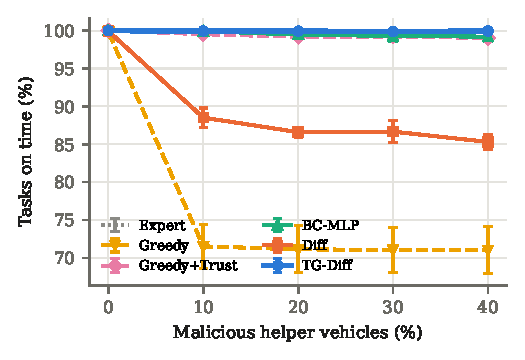
\includegraphics[width=\columnwidth]{figures/fig_malicious.pdf}
\caption{Tasks completed on time versus the share of malicious helper vehicles, with a black-hole RSU and false state reports (mean $\pm$ std, 3 seeds).}
\label{fig:malicious}
\end{figure}

\subsection{Data Poisoning}
Fig.~\ref{fig:poison} retrains the learned policies on data in which a fraction $\rho$ of the samples offering a malicious option are relabelled to it, and evaluates them with 30\% malicious helpers. Trust \emph{inputs} alone do not protect a learned policy against poisoning: BC-MLP falls from 99.3\% to 91.2\% as $\rho$ grows to 30\%. \tgd{} stays between 98.7\% and 99.7\%, because the guidance term suppresses untrusted targets at decision time whatever the denoiser learned.

\begin{figure}[t]
\centering
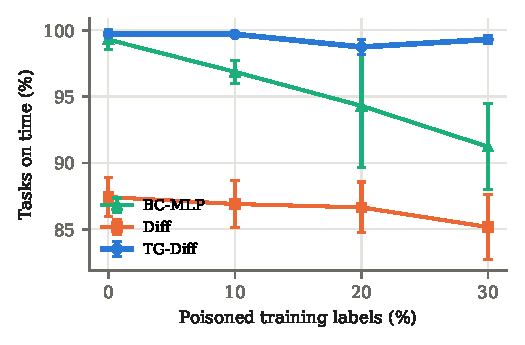
\includegraphics[width=\columnwidth]{figures/fig_poison.pdf}
\caption{Tasks completed on time versus the share of poisoned training labels, with 30\% malicious helpers (mean $\pm$ std, 3 seeds).}
\label{fig:poison}
\end{figure}

\subsection{Decision Time}
Fig.~\ref{fig:steps} varies the number of DDIM steps $K$. The measured decision time on a two-core CPU grows from 0.19~ms at $K=1$ to 2.34~ms at $K=20$, small compared with deadlines of 0.4--1~s. Success barely depends on $K$ in this discrete setting (99.2--99.9\% for \tgd{}), so few steps suffice; richer action spaces may need more.

\begin{figure}[t]
\centering
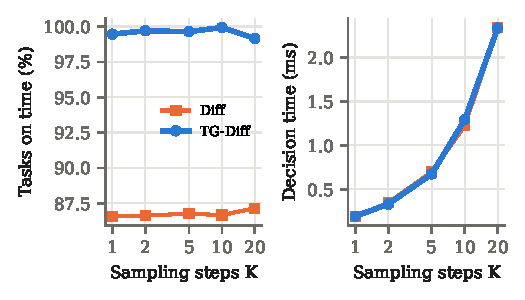
\includegraphics[width=\columnwidth]{figures/fig_steps.pdf}
\caption{Effect of the number of sampling steps $K$ on tasks completed on time (left) and on the measured decision time (right), with 30\% malicious helpers.}
\label{fig:steps}
\end{figure}

\subsection{Ablation and Value of the Digital Twin}
Table~\ref{tab:ablation} removes one component at a time with 30\% malicious helpers and 20\% poisoned labels. Trust guidance is the decisive component: without it, success falls from 99.0\% to 91.7\%. Removing the trust input costs 1.2 points and adds 33~ms of latency.

\begin{table}[t]
\caption{Ablation with 30\% malicious helpers and 20\% poisoned labels}\label{tab:ablation}
\centering\footnotesize
\begin{tabular}{@{}lccc@{}}
\toprule
Variant & On time (\%) & Latency (ms) & Lost tasks \\ \midrule
\tgd{} (full) & 99.0 $\pm$ 0.4 & 191 & 2 \\
without trust input & 97.8 $\pm$ 1.2 & 224 & 0 \\
without trust guidance & 91.7 $\pm$ 3.4 & 169 & 169 \\
without digital twin & 98.9 $\pm$ 0.5 & 211 & 0 \\
Diff (no trust) & 85.4 $\pm$ 2.2 & 180 & 300 \\
\bottomrule
\end{tabular}
\end{table}

In this setting the twin brings no gain in success, because malicious nodes also drop tasks and the beta reputation detects them. To isolate the twin, we ran a second scenario in which malicious nodes \emph{only} lie about their queues and never drop tasks, under heavy load (1 task per vehicle per second). Behaviour-based trust cannot see these nodes: Greedy+Trust without the twin completes 74.0\% (60 vehicles) and 78.0\% (80 vehicles) of the tasks, with mean latencies of 2.7~s and 3.5~s caused by congestion at the lying nodes. With the twin, the same heuristic reaches 100\% at 173 and 180~ms, and \tgd{} reaches 100\% at 172 and 170~ms against 198~ms without the twin.

\subsection{Discussion and Limitations}
Three findings stand out. First, an unprotected diffusion policy is markedly more vulnerable than a trust-aware heuristic, which confirms that generative decision makers are an attack surface. Second, trust must act \emph{inside} the generative process: trust features alone do not survive data poisoning, guidance does. Third, the twin is necessary against nodes that lie without dropping tasks. The prototype has limits that the full study will address: a synthetic highway instead of SUMO traces, a discrete action space in which a trust-aware heuristic is already strong, behaviour cloning instead of critic-based training, a single training seed, and attacks that do not adapt to the defense (e.g., nodes that build trust before attacking). \todo{campagne complète avec SUMO, 5 graines d'entraînement, attaquants adaptatifs}


% ===========================================================================
\section{Conclusion}\label{sec:conclusion}
We showed that a diffusion policy for vehicular offloading is a target in its own right, and proposed \tgd{}, which places trust inside the denoising process and uses a digital twin to expose nodes that lie about their state. \resConclusion{} Future work will (i) evaluate \tgd{} on SUMO mobility traces of a real road network~\cite{lopez2018sumo}, (ii) fine-tune the policy with a learned critic~\cite{wang2023diffusionql} and extend the action to joint target selection and resource allocation, where generative policies are expected to outperform discrete heuristics, and (iii) protect the confidentiality of offloaded generative workloads with lightweight homomorphic encryption~\cite{elbouabidi2026hybrid_he}.

\bibliographystyle{IEEEtran}
\bibliography{refs}

\end{document}
